\chapter{Реализация и экспериментальная проверка}

\begin{annotation}
	В данной главе приводятся детали разработки и экспериментальной проверки
	разработанной системы. Описан выбор инструментов, используемых для реализации
	программного обеспечения. Приводится выбор инфраструктурных решений,
	с учетом поставленных ранее системных и функциональных требований.
	Описаны состав и структура реализованного программного обеспечения.
\end{annotation}


% todo можно привести таблицу AKAIKE с разными гиперпараметрами для


\section{Выбор инструментальных средств}

В качестве языка программирования для проведения экспериментов и анализа данных
будет использоваться python. Это язык с динамической типизацией, но зато с
большим количеством хорошо протестированных и отлаженых библиотек для работы
с данными (numpy, pandas), статистическим анализом (statmodels) и фреймфорками для построения нейросетей (pytorch, tensorflow).

Для распараллеливания работы с данными и использовании аппаратных ускорений для умножений матриц
для реализации модуля подсистемы обработки данных и подсистемы для вычисления нечеткой карты
будет использоваться pytorch. Это фреймворк для работы с данными и созданию нейросетей.

Конкурентом pytorch является tensorflow, но за счет того, что в pytorch не статический
граф вычислений, а динамический, pytorch предоставляет больше свободы, но и больше мест,
где можно ошибиться.

Недостатком python можно считать динамическую типизацию. Динамическая типизация не позволяет
найти многие ошибки на стадии компиляции. Многие ошибки можно обнаружить только во время
работы программы. Для того, чтобы бороться с этим недостатком, вместе с кодом нужно писать
автоматические тесты --- они позволяют быстро проверить работоспособность программы.

\section{Состав и структура реализованного программного обеспечения}
\begin{annotation}
	В данном разделе рассматривается состав ия структура реализованного программного обеспечения.
	Приводятся характеристики разработанного программного продукта, возможности конфигурации отдельных
	компонент системы. Описано назначение исполняемых файлов, описаны требования к системному окружению.
\end{annotation}

Реализованное по --- это модуль на python, который позволяет помочь эксперту
исследовать моделируемую систему и структурировать знания о системе.

Так как разработка проводилась с методикой Test-Driven-Development,
также были написаны автотесты, которые запускаются
при обновлении кода в удаленном репозитории. Кроме автотестов,
в среде по запуску тестов проверяется качество кода и возможные ошибки
с помощью линтеров на соответствие кода стандарту pep8.
Автотесты необходимы проекту на языке с динамической типизацией,
так как в интерпретируемых языках с динамической типизацией
интерпретатор на стадии компиляции программы не может проверить или вывести, чтобы проверить
типы переменных и аргументов функций самостоятельно. Поэтому код, который
не покрыт тестами может не работать и об этом разработчик узнает
только после того, как программа упадет. Но раннее обнаружение этих
ошибок с помощью автотестов поможет избежать проблем с использованием модуля в
продакшне и поможет сократить время доведения продукта до состояния успешного релиза.

\section{Анализ данных}

Набор данных, на которых будет проводиться тестирование разработанной системы
представляет из себя несколько $ csv $ файлов: файл с количеством продаж
продуктов разных категорий в 3 магазинах за 5 лет начиная с 29.01.2011
и файл с описанием праздников, которые выпадают на каждый день.

Требуется предсказать количество продаж на 30 дней вперед.

Для начала можно провести качественный визуальный анализ данных.

Общее количество продаж можно оценить на графике \ref{img:all_sales}.
Из этого графика видно, что до середины 2012 года количество проданных
товаров увеличивалось. Но после тренд пропал. В данных можно наблюдать
как годичные, так и месячные и даже недельные сезонности. Каждый год
в Рождество количество проданных товаров равно 0, потому что магазин не работает.
По выходным количество проданных товаров больше, чем в будние дни.

Количество проданных товаров по каждому магазину представлено на следующем графике \ref{img:sales_by_store}.
В количестве проданных товаров отдельно по каждому магазину нет значительных отличий.
Все магазины продают примерно одинаковое количество товаров.

Количество продаж по категориям для каждого магазина на графику \ref{img:sales_by_store_by_cat}
Во всех трех магазинах количество продаж товаров в категории "еда" больше всего,
а товаров для дома меньше всего. Из данного графика можно заметить, что сезонность
присутствует в графике по продаже товаров в категории "еда" и для товаров для дома, но
для товаров для хобби сезонности не наблюдаются.

Рассмотрим графики автокорреляции и частичной автокорреляции для общего количества продаж
\ref{img:any_autocorrelation}.
Для лагов 1, 2, 3, 6, 7 присутствует статически значимая частичная автокорреляция.
Это может быть использовано при построении модели SARIMAX.
На графики автокорреляции видны синусоидельные колебания. Это свидетельствует и подтверждает,
что в данных есть сезонность.

\def\figurename{Рис}
\begin{figure}[t]
	\centering
	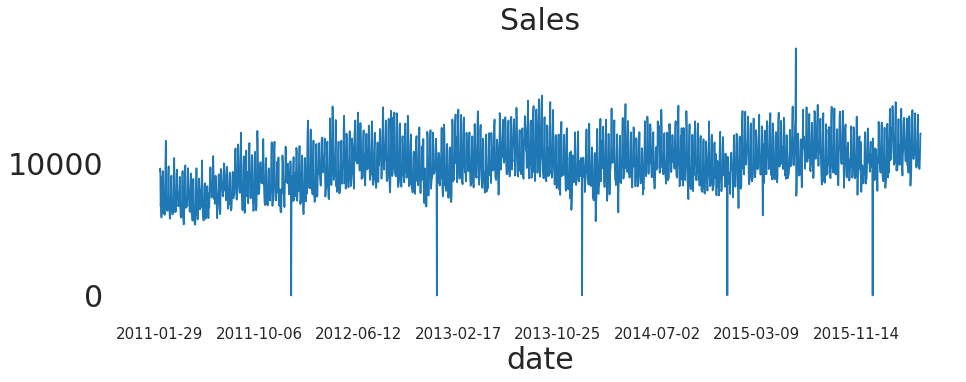
\includegraphics[width=0.9\columnwidth]{./img/all_sales.png}
	\caption{Количество продаж}
	\label{img:all_sales}
\end{figure}


\def\figurename{Рис}
\begin{figure}[t]
	\centering
	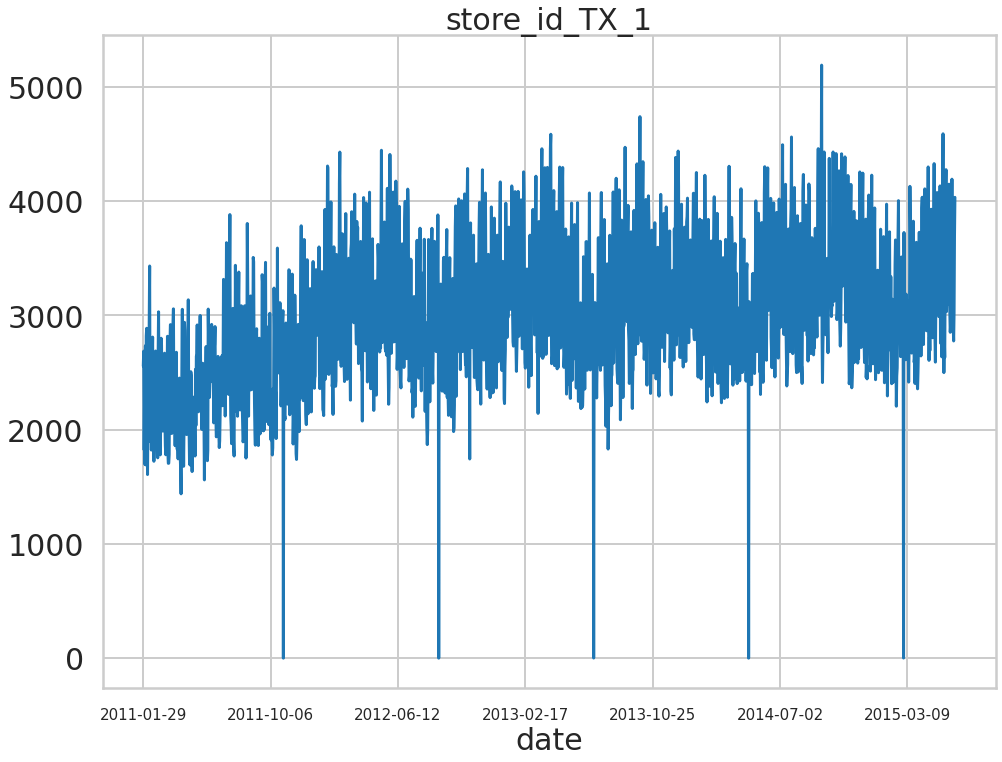
\includegraphics[width=0.25\columnwidth]{./img/store_tx1_total.png}
	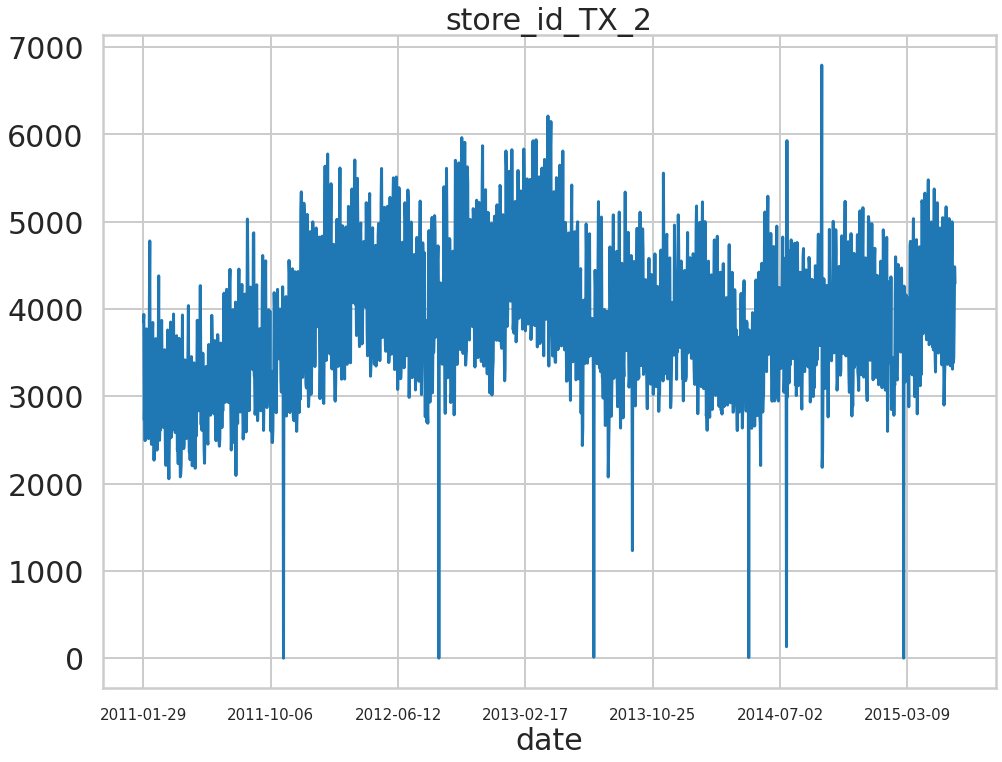
\includegraphics[width=0.25\columnwidth]{./img/store_tx2_total.png}
	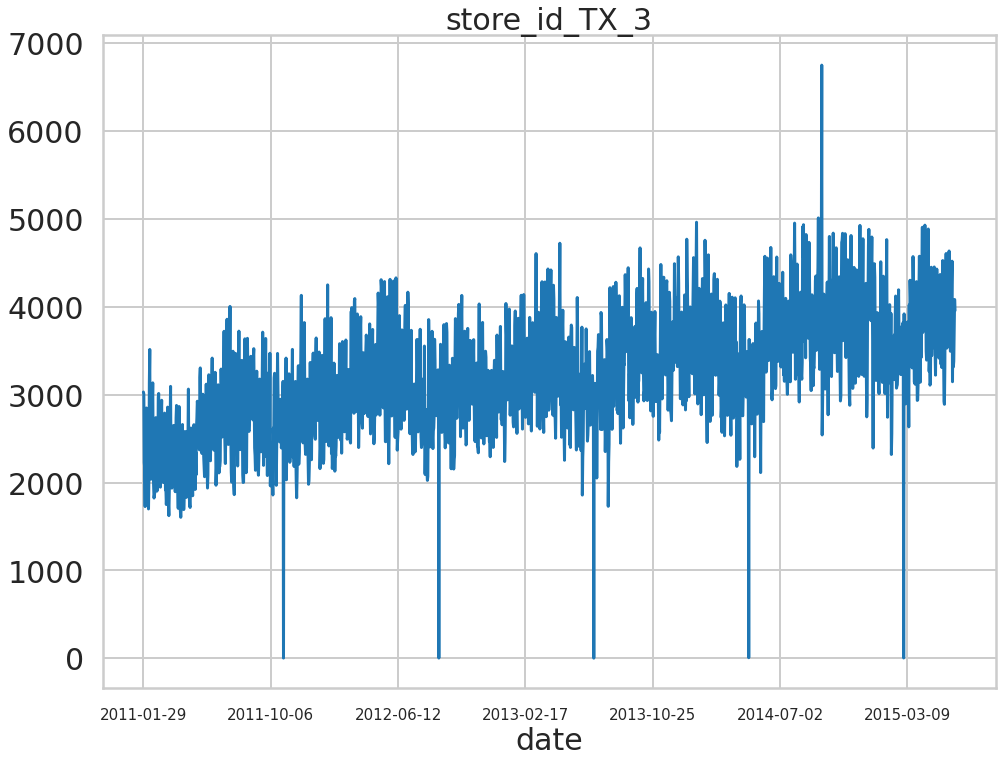
\includegraphics[width=0.25\columnwidth]{./img/store_tx3_total.png}
	\caption{Общее количество продаж по каждому магазину}
	\label{img:sales_by_store}
\end{figure}

\def\figurename{Рис}
\begin{figure}[t]
	\centering
	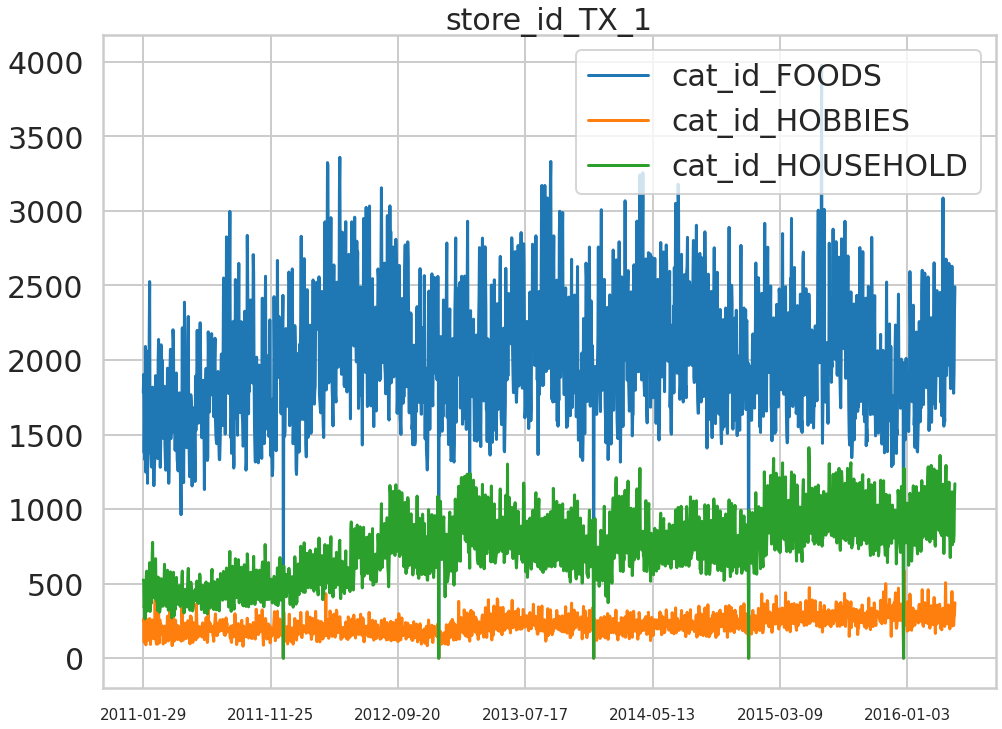
\includegraphics[width=0.25\columnwidth]{./img/store_tx1_by_cats.png}
	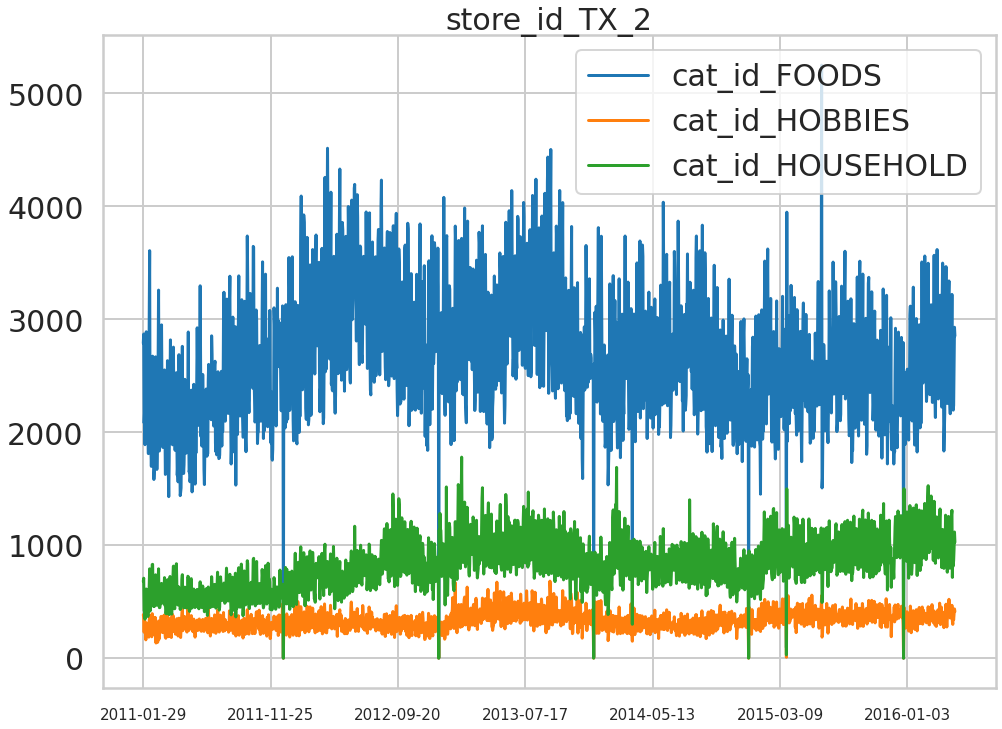
\includegraphics[width=0.25\columnwidth]{./img/store_tx2_by_cats.png}
	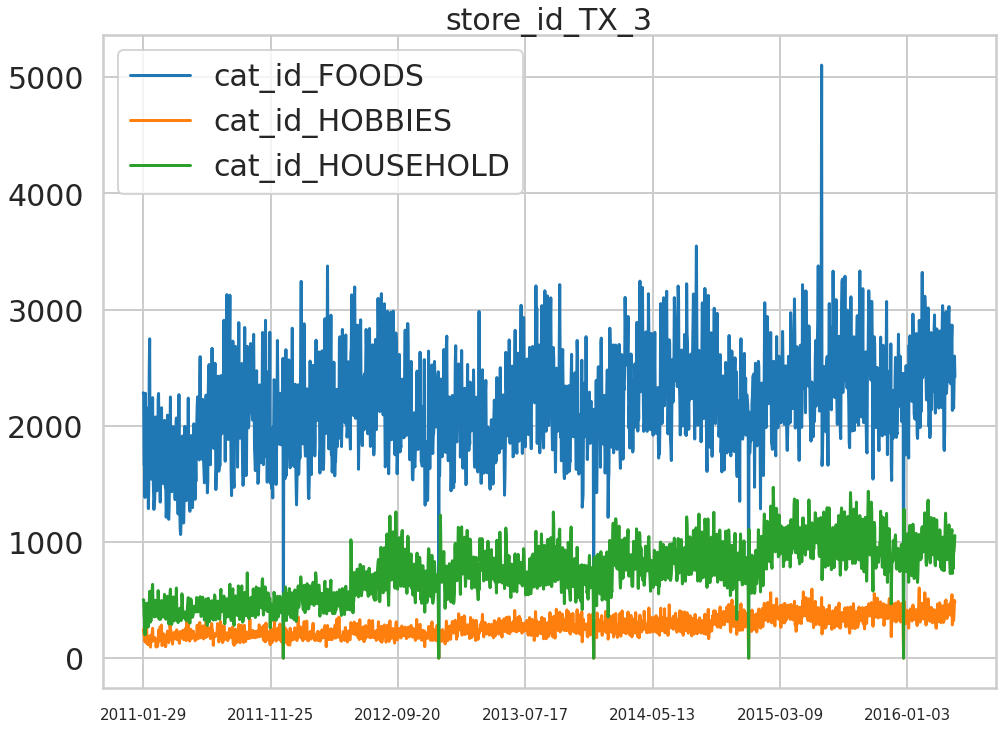
\includegraphics[width=0.25\columnwidth]{./img/store_tx3_by_cats.png}
	\caption{Количество продаж товаров определенной категории для каждого магазина}
	\label{img:sales_by_store_by_cat}
\end{figure}

\def\figurename{Рис}
\begin{figure}[t]
	\centering
	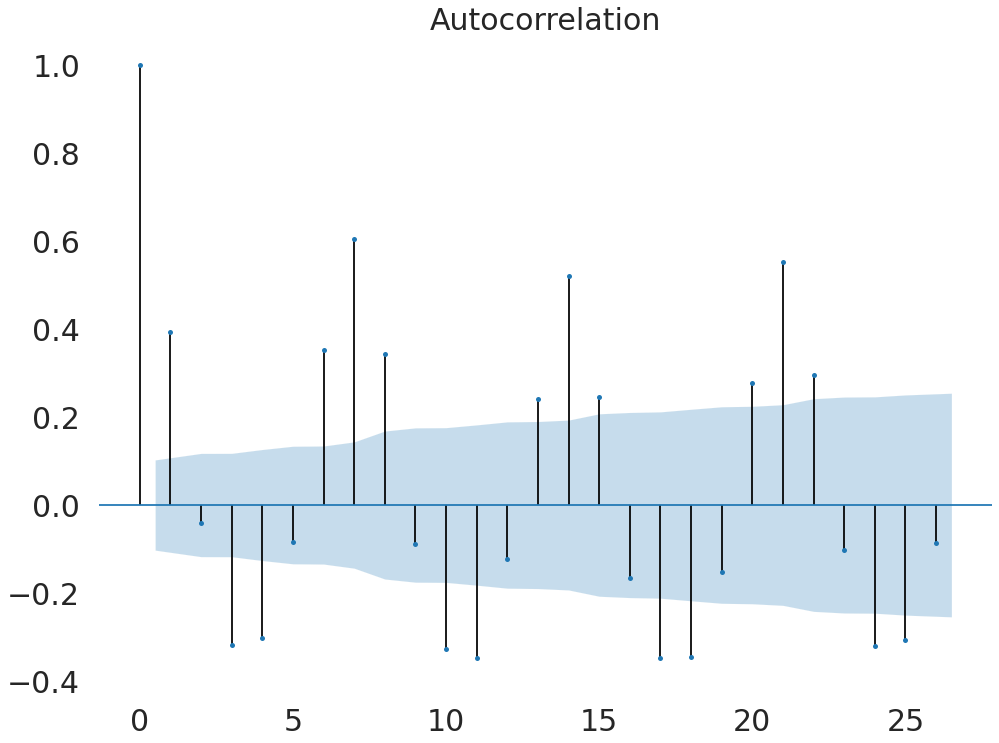
\includegraphics[width=0.4\columnwidth]{./img/sales_autocorrelation.png}
	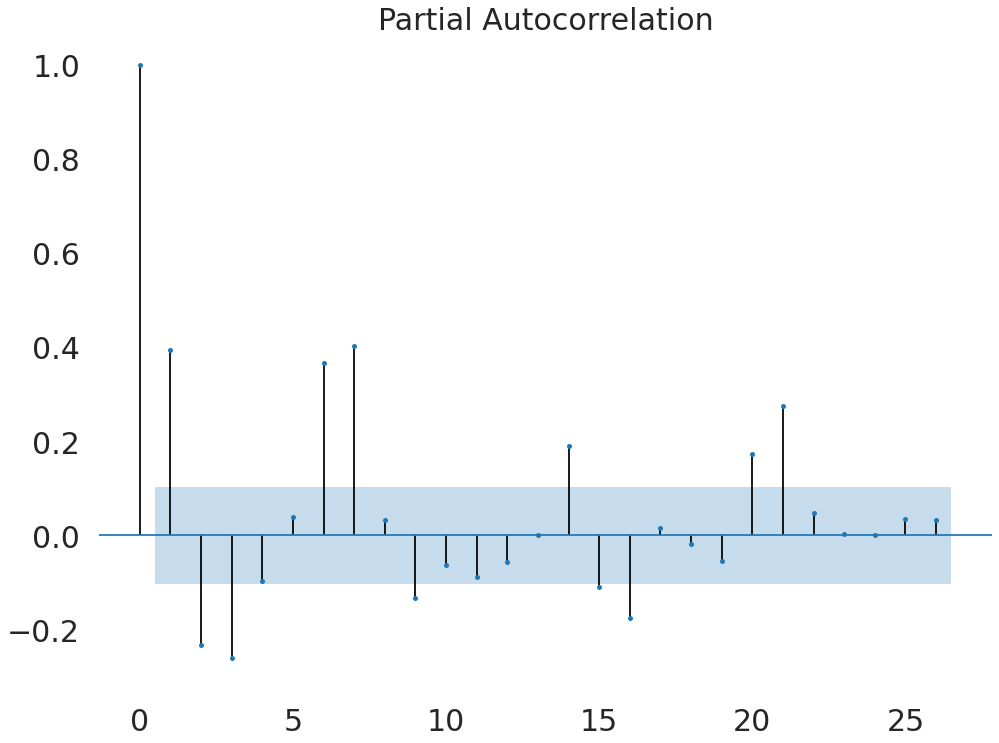
\includegraphics[width=0.4\columnwidth]{./img/sales_partial_autocorrelation.png}
	\caption{Автокорреляция и частичная автокорреляция для общего количества продаж}
	\label{img:any_autocorrelation}
\end{figure}



\section{Построение модели SARIMAX}

Для оптимального подбора гиперпараметров был проведен
визуальный анализ исходных данных, а так же проведена
кросс-валидация с поиском модели с минимальным значением критерия Акаике \cite{akaike}.
Оптимизация параметров на полном наборе данных занимает примерно 10 секунд при 8 параметрах модели.

Оптимальными гиперпараметрами оказались:
$ p = 2, d = 0, q = 3, P = 0, D = 1, Q = 1, S = 7 $.
Сезонность недельная  -~ это логично, что в текущий день
товаров будет продано столько же, как неделю назад.

На графике остатков \ref{img:arimax_resid} все еще прослеживается
годичная сезонность и выбросы. Выбросы -~ предсказать возможно, если
добавить экзогенные параметры в виде индикатора праздников.

В качестве экзогенных параметров рассмотрим индикатор дня недели.
В исходные данные добавится 7 колонок. Каждому дню недели
будет соответствовать одна колонка. И еще одним экзогенным параметром
возьмем индикатор праздника -- Рождества.
Экзогенные параметры можно вычислить заранее, так как наперед можем
поставить в соответствие индикатор дня недели определенному календарному дню
и индикатор Рождества.
Оптимизация параметров модели с 8 экзогенными переменными потребовало 20 секунд.

На графике остатков модели с экзогенными переменными \ref{img:arimax_resid} видно, что удалось избавиться
от большого значения остатков на Рождество. Это получилось сделать благодаря
столбцу-индикатору Рождественских праздников.

\def\figurename{Рис}
\begin{figure}[t]
	\centering
	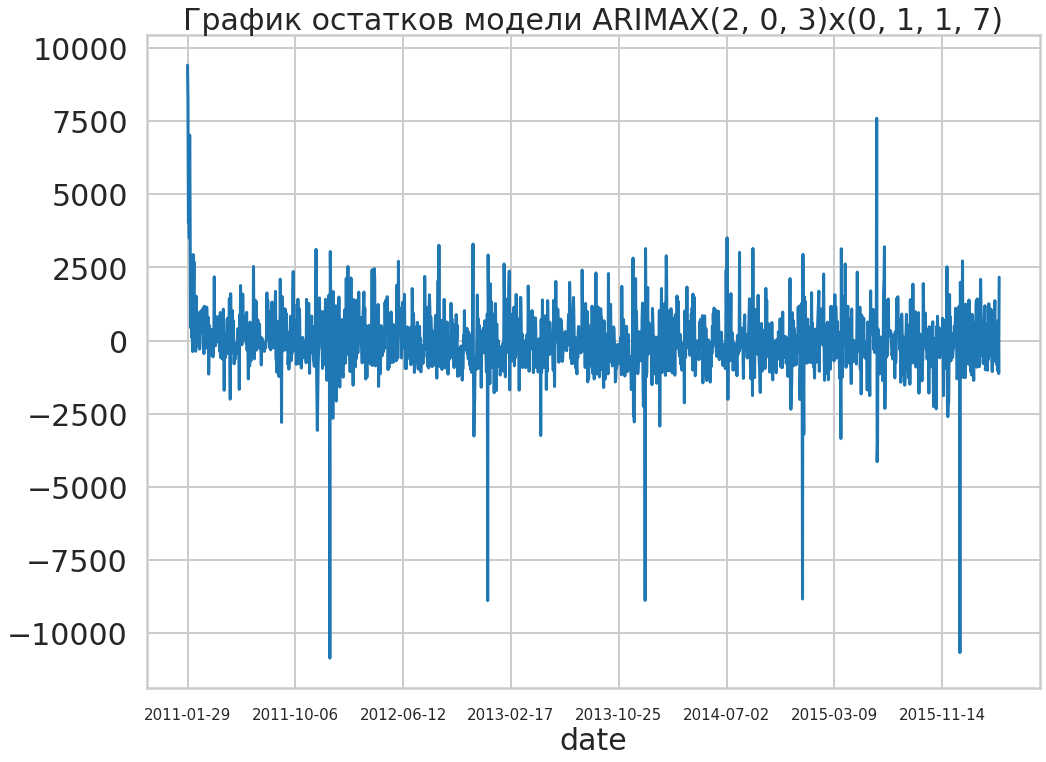
\includegraphics[width=0.4\columnwidth]{./img/arimax_resid.png}
	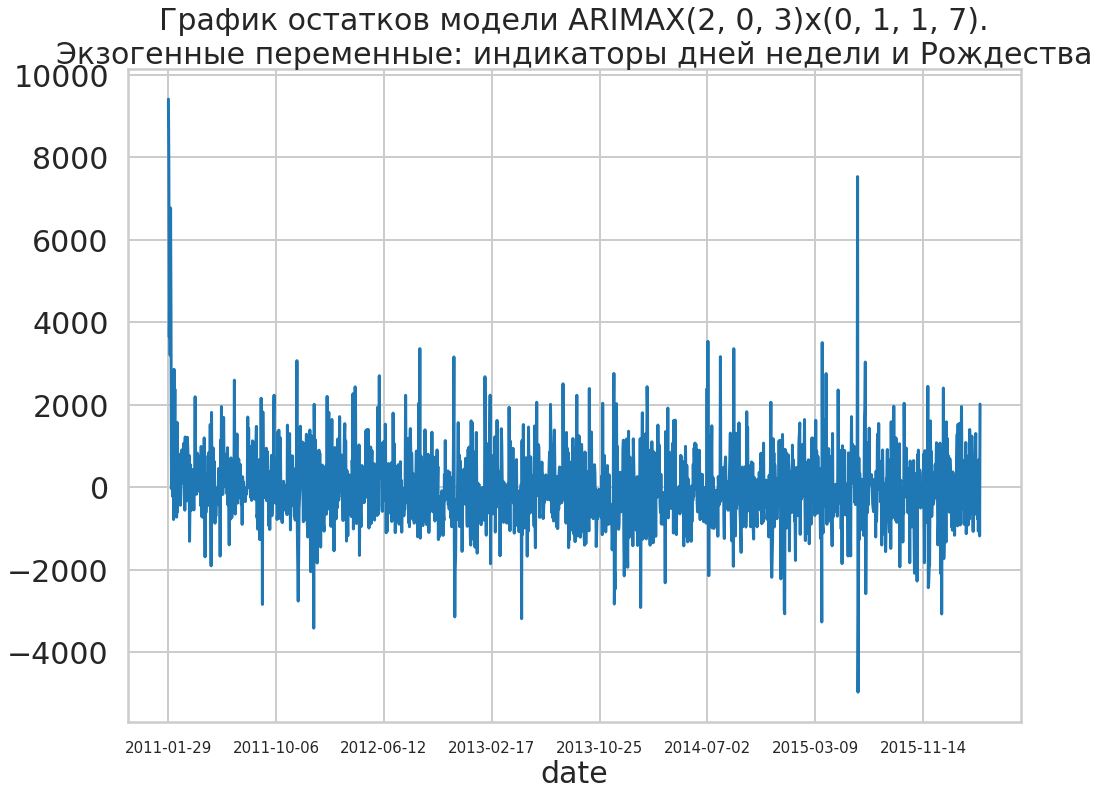
\includegraphics[width=0.4\columnwidth]{./img/arimax_resid_with_xmas.png}
	\caption{График остатков модели ARIMAX с соответствующими параметрами}
	\label{img:arimax_resid}
\end{figure}

Но если проанализировать значения коэффициентов обученной модели \ref{tbl:arimax_coeffs_exogen},
можно заметить, что индикаторы дня недели слишком слабо влияют на предсказание модели.
Значения коэффициентов очень маленькие, вероятность того, что эти параметры будут иметь
значение больше критического равно единице, дисперсия большая. Из этого можно сделать вывод,
что использование этих экзогенных переменных неоправданно. Но зато значение коэффициента
для индикатора Рождества ($ xmas $) большое. Этот экзогенный параметр
действительно объясняет некоторую полезную часть данных. Так, значение теста Харке-Бера
для предыдущей модели было равно $ 37658.88 $, а после выявления зависимости между количеством продаж
и днем рождества стало равно $ 1488.02 $. Чем ближе значение этого теста к нулю, тем больше остатки
модели похожи на нормальное распределение. Этот тест сверяет асимметрию и эксцесс остатков с
значениями этих моментов для нормального распределения. И хотя с таким абсолютным значением
теста нельзя говорить о том, что остатки распределены нормально, но относительно предыдущей
модели, новая модель определенно лучше.

Но на предсказании на 30 дней вперед найденные экзогенные переменные не повлияли \ref{img:arimax_forecast},
так как в исследуемый момент времени не было Рождества.

\def\figurename{Рис}
\begin{figure}[t]
	\centering
	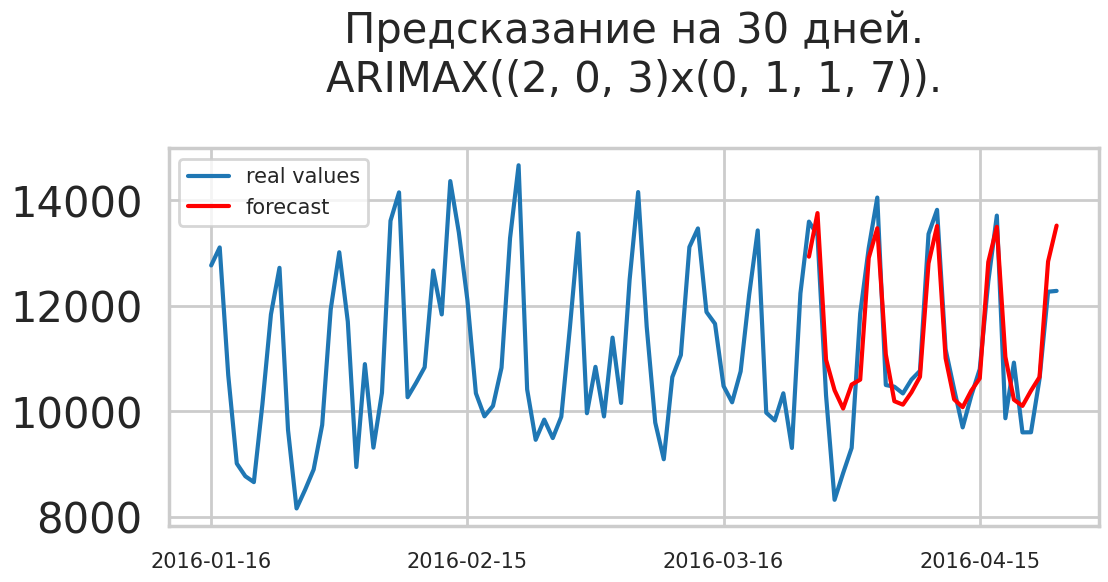
\includegraphics[width=0.9\columnwidth]{./img/arimax_simple_pred30.png}
	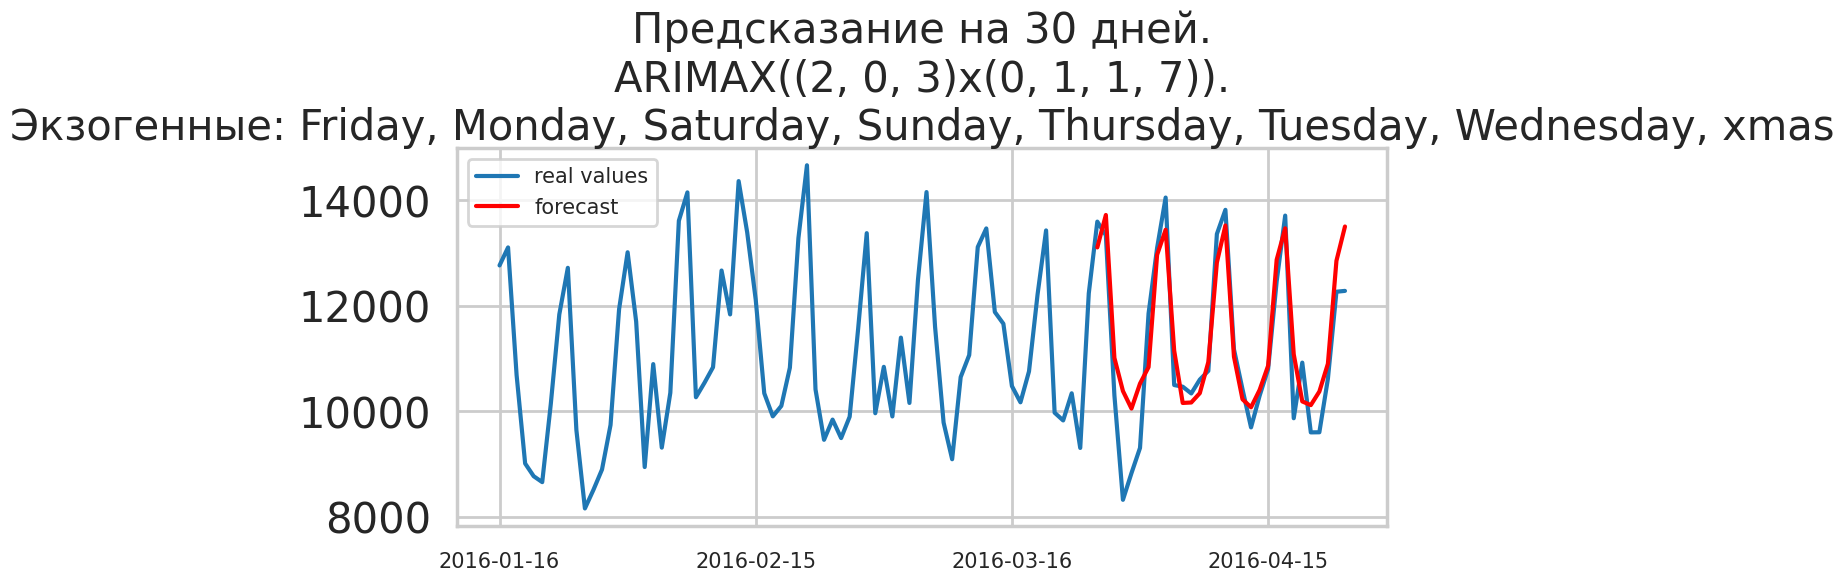
\includegraphics[width=0.9\columnwidth]{./img/arimax_with_exog_pred30.png}
	\caption{Предсказания на 30 дней вперед}
	\label{img:arimax_forecast}
\end{figure}

Значение $ RMSSE $ для модели с экзогенными параметрами ($ RMSSE = 0.000210 $) незначительно меньше
модели без экзогенных переменных ($ RMSSE = 0.000208 $).


\section{Построение модели LSTM}

В отличие от таких статистических методов как ARIMAX, предсказание данных
с помощью нейросетей требует более тщательно предобработки данных.
Перед тем, как скормить данные на вход нейросети, их нужно нормализовать.
Для того, чтобы нормализовать данные, вычтем из данных за каждый день средннее
количество продаж и разделим на стандартное отклонение. После того, как
нейросетевая модель посчитает предсказание, полученные в предсказании
числа нужно будет умножить на стандартное отклонение и прибавить среднее.
Важно, чтобы обучающая выборка была репрезентативной. Так как модель
может вести себя неадекватно, если входные данные слишком сильно отличаются
от данных, которые были на обучающей выборке.

К сожалению, предсказания, которые мы получили с помощью  LSTM менее интерпретируемы,
чем те, которые мы получили с помощью SARIMAX. Однако LSTM --- это намного более
мощная модель. И может быть использована в тех случаях, если мощности SARIMAX не хватает.
Также можно использовать эти модели вместе. Например, сначала с помощью SARIMAX создать
модель, которую можно интерпретировать, а потом с помощью LSTM можно предсказывать остатки, которые будет
давать SARIMAX. И эти остатки можно прибавлять к исходному предсказанию SARIMAX. Такой алгоритм
не позволит повысить интерпретируемость предсказания, но позволит увеличить его точность.

Результаты предсказаний с помощью модели LSTM очень похожи на результаты предсказаний
с помощью SARIMAX. Стоит заметить, что LSTM была обучена и вычислялась с помощью GPU.
В то время как оптимизация параметров модели SARIMAX производились на процессоре и
для получения примерно одинаковых результатов требовалось столько же времени.
Если бы LSTM обучалась на процессоре, время обучения бы исчислялось не секундами, а часами,
так как это затратный по вычислительным мощностям процесс.

В результате эксперимента была обучена LSTM сеть с размерностью скрытого слоя равной 200.
Результат обработки LSTM-сети после ее вычислений попадал в полносвязную сеть с размерностью
тоже 200. Кривая потерь в процессе обучения и график с предсказаниями представлены не графиках \ref{img:lstm_forecast}.
Значение $ RMSSE = 0.000167 $. Это немного меньше, чем у модели SARIMAX, но незначительно.

\def\figurename{Рис}
\begin{figure}[t]
	\centering
	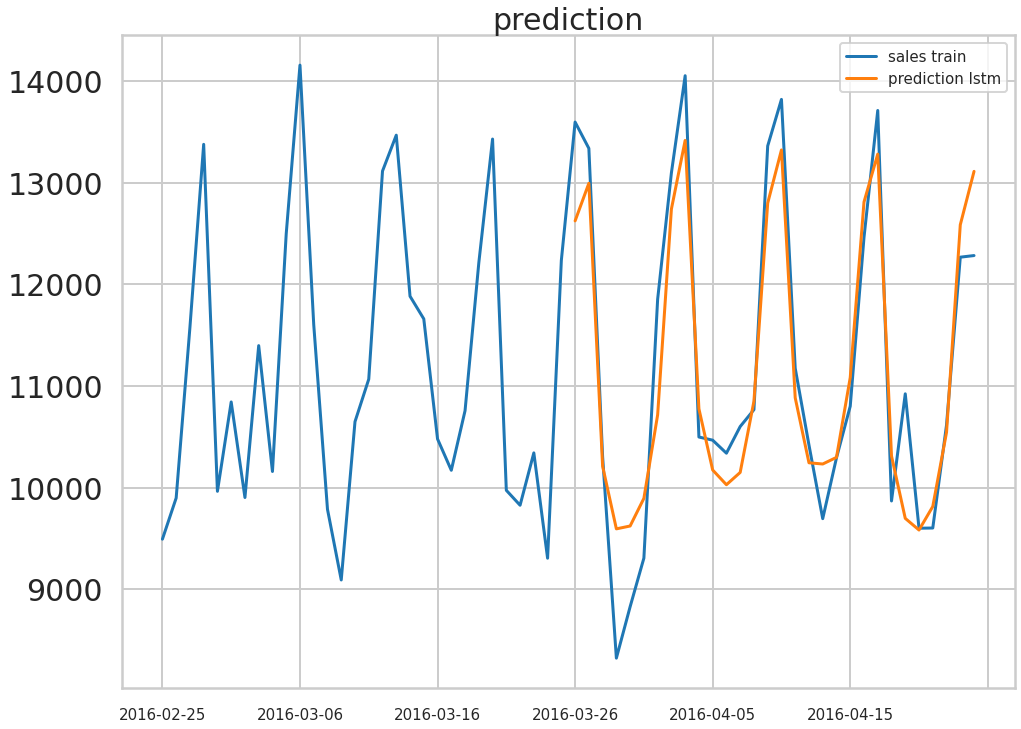
\includegraphics[width=0.4\columnwidth]{./img/lstm_prediction.png}
	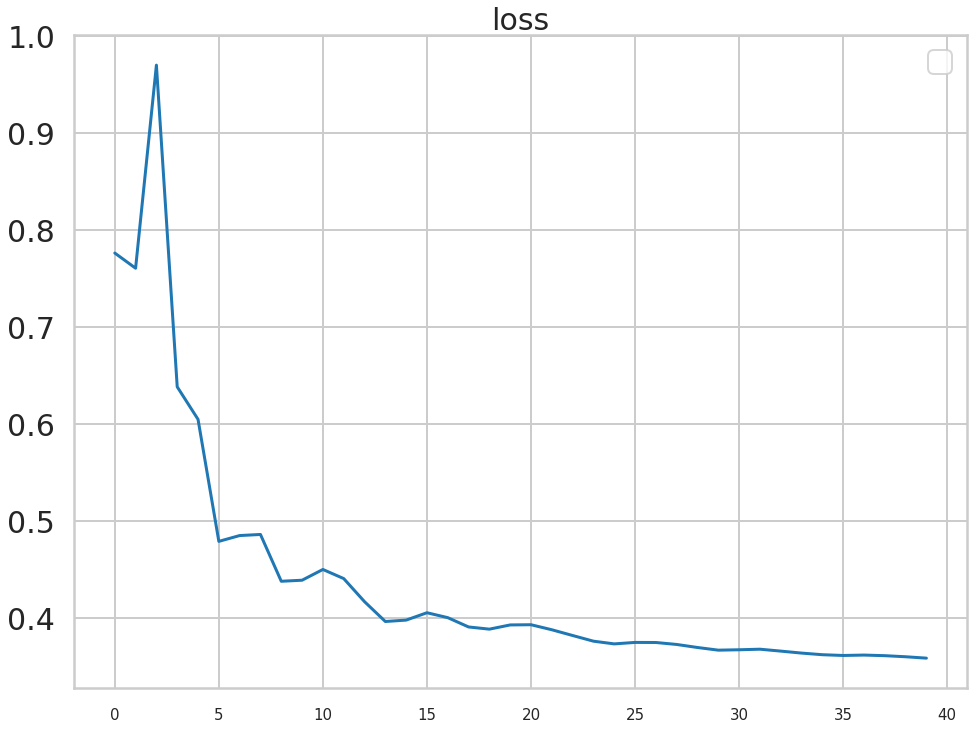
\includegraphics[width=0.4\columnwidth]{./img/lstm_loss.png}
	\caption{Кривая потерь и предсказание LSTM-сети}
	\label{img:lstm_forecast}
\end{figure}

\section{Построение модели FCM}


% \section{Тестирование разработанной системы}

% Для тестирования системы были построены 3 варианта карты:
% \begin{itemize}
% 	\item Карта без связей.
% 	\item Полносвязная карта.
% 	\item Карта с осмысленными связями.
% \end{itemize}

% Все карты обучались 100 эпох, имели размерность скрытого состояния 100,
% количество исторических данных, обрабатываемых с помощью LSTM на одной итерации -~ 100.
% Так же как и количество данных на выходе, сгенерированных.

% Карта без связей \ref{img:lstmfcm_empty}, обученная на тестовых данных
% показала отличный результат для $ x_1, x_2, x_3, x_4  $. Однако ошибка
% для $ x_5, y $ довольно велика. Такие предсказания эквивалентны предсказаниям
% отдельно взятых моделей LSTM, обученных для предсказания временного ряда
% по истории только этого временного ряда.

% Карта, которая представляет из себя полносвязный граф \ref{img:lstmfcm_fc},
% из-за избыточности связи получила предсказания для $ x_1, x_2, x_3 $ даже
% хуже, чем карта без связей. Это можно объяснить излишней сложностью модели.
% Модель слишком усложнена и не может обучиться за заданное количество эпох.

% Карте с осмысленными связями \ref{img:lstmfcm_meaningful} удалось сохранить качество
% предсказаний для $ x_1 --- x_4 $ таким же, как и у карты без связей.
% А так же удалось получить улучшение предсказания для $ y $.
% Неожиданный результат получили для $ x_5 $. todo как так?

% Для карт, у которых были связи с $ x_5, y $ получилось лучше предсказать значения
% для этих рядов. Потому что значения этих рядов зависят от $ x_1 --- x_4 $.

% Кроме того, на долгосрочных предсказаниях видно, что $ x_4 $ имеет проседания.
% Вероятно, это связано с ограничениями, рассмотренными во второй главе.
% Так как модель обучается на одних данных, а после предсказания, модель возвращает
% данные в новой области значений, будущие предсказания становятся все более нестабильными.
% todo не понятно, почему их нет на предсказании LSTM

% \def\figurename{Рис}
% \begin{figure}[t]
% 	\centering
% 	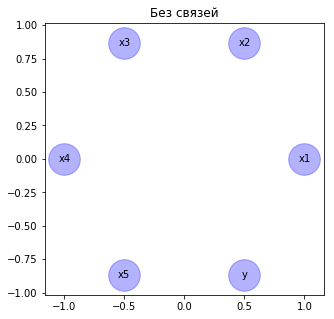
\includegraphics[width=0.7\columnwidth]{./img/lstmfcm_empty.png}
% 	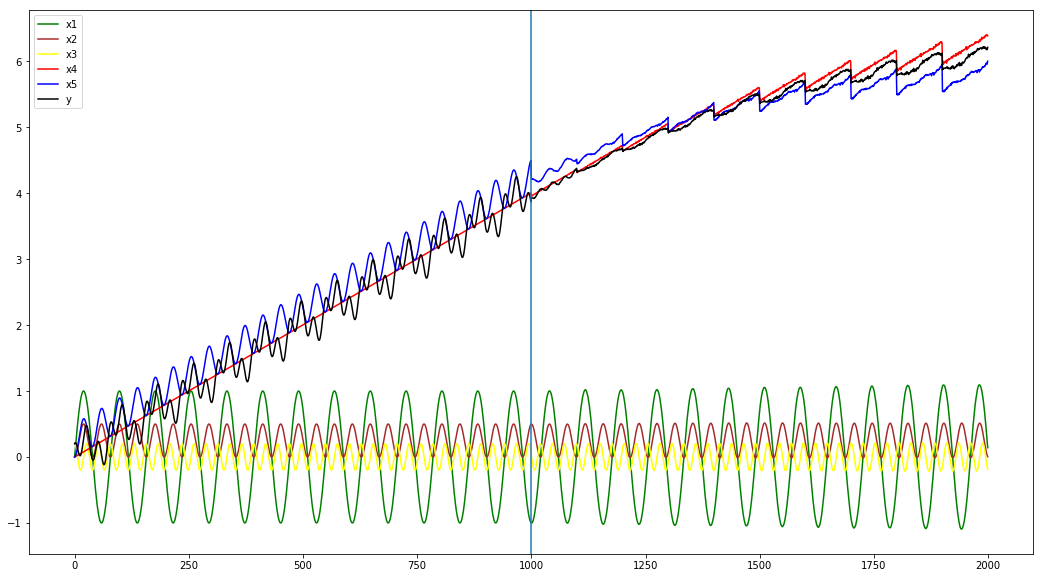
\includegraphics[width=0.9\columnwidth]{./img/lstmfcm_empty_prediction.png}
% 	\caption{Карта без связей концептов}
% 	\label{img:lstmfcm_empty}
% \end{figure}

% \begin{figure}[t]
% 	\centering
% 	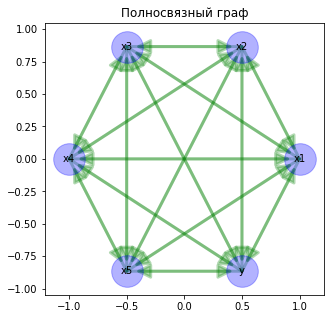
\includegraphics[width=0.7\columnwidth]{./img/lstmfcm_fc.png}
% 	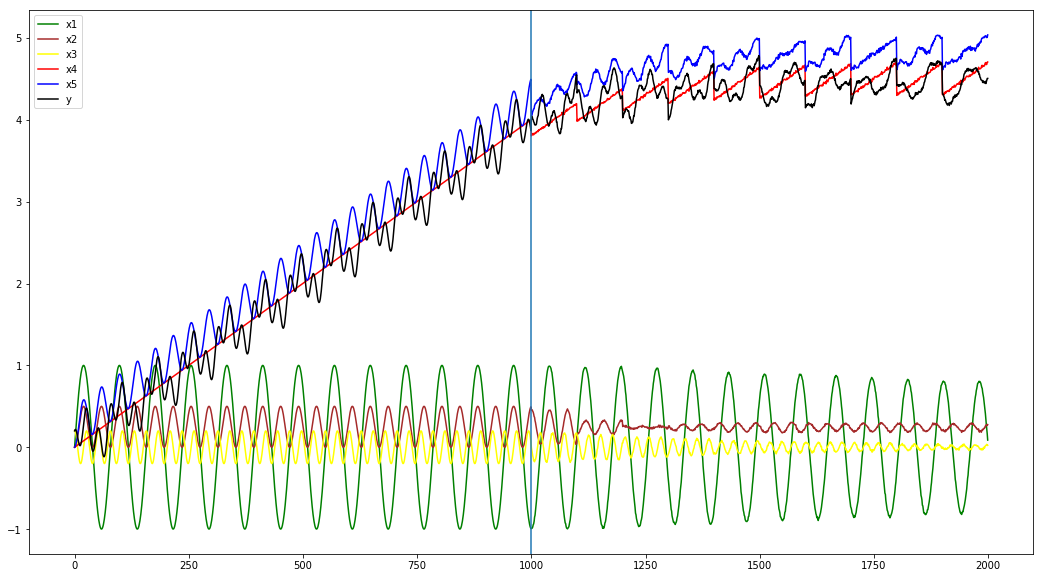
\includegraphics[width=0.9\columnwidth]{./img/lstmfcm_fc_prediction.png}
% 	\caption{Полносвязная карта}
% 	\label{img:lstmfcm_fc}
% \end{figure}

% \begin{figure}[t]
% 	\centering
% 	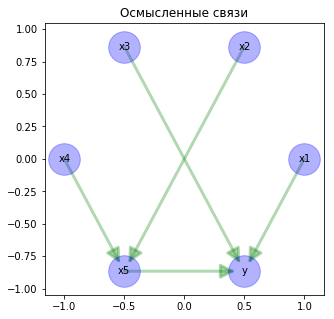
\includegraphics[width=0.7\textwidth]{./img/lstmfcm_meaningful.png}
% 	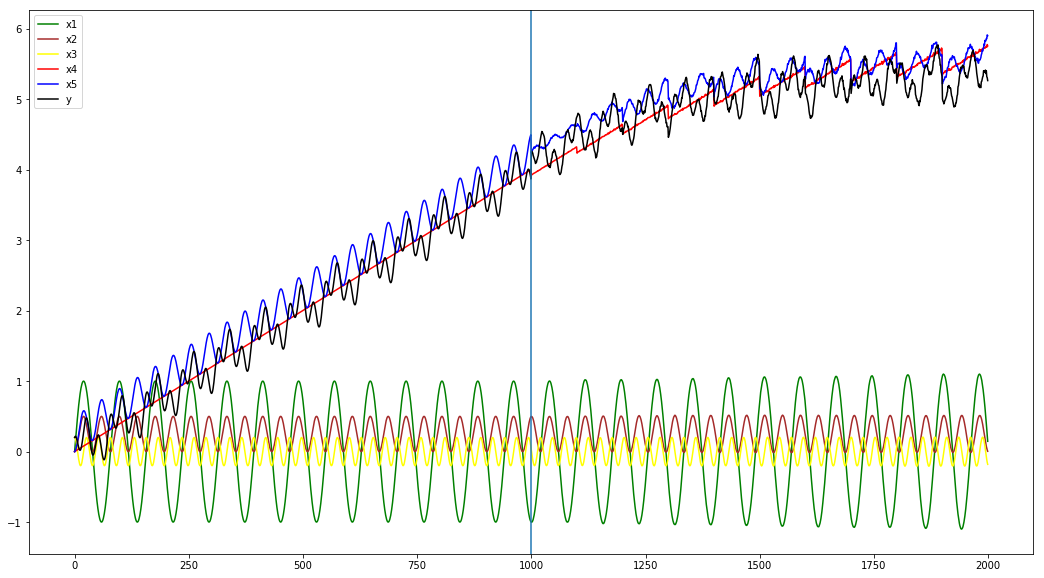
\includegraphics[width=0.9\textwidth]{./img/lstmfcm_meaningful_prediction.png}
% 	\caption{Карта с осмысленно расставленными связями}
% 	\label{img:lstmfcm_meaningful}
% \end{figure}


% \section{Экспериментальное сравнение разработанной системы с существующими}

% Была построена модель, основанная на LSTM,
% которая одновременно анализирует все временные ряды тестовых данных.

% Результат предсказаний такой модели представлен на рисунке \ref{img:lstm_only_prediction}.
% Результат зашумлен по сравнению с предсказаниями карты (todo не могу объяснить).
% И в отличие от карты, даже с осмысленными связями, на этом предсказании не наблюдается скачков
% между итерациями предсказаний. И $ x_5 $ тоже удалось предсказать относительно успешно.

% Данная модель так же, как и карта работала рекурсивно:
% на каждой следующей итерации обрабатывала данные, полученные на предыдущей.
% Скачок вначале предсказаний, скорее всего, связан с тем, что после обучения,
% скрытое состояние сети выставляется заново, так как меняется его размерность.
% Возможно, использование скрытого состояния одинаковой размерности во время
% тренировки и во время тестирования, может избавить от этой проблемы. Однако
% в LSTM NFCM между итерациями тоже сохраняются эти скачки, хотя между итерациями
% скрытое состояние не переинициализируется.

% \begin{figure}[t]
% 	\centering
% 	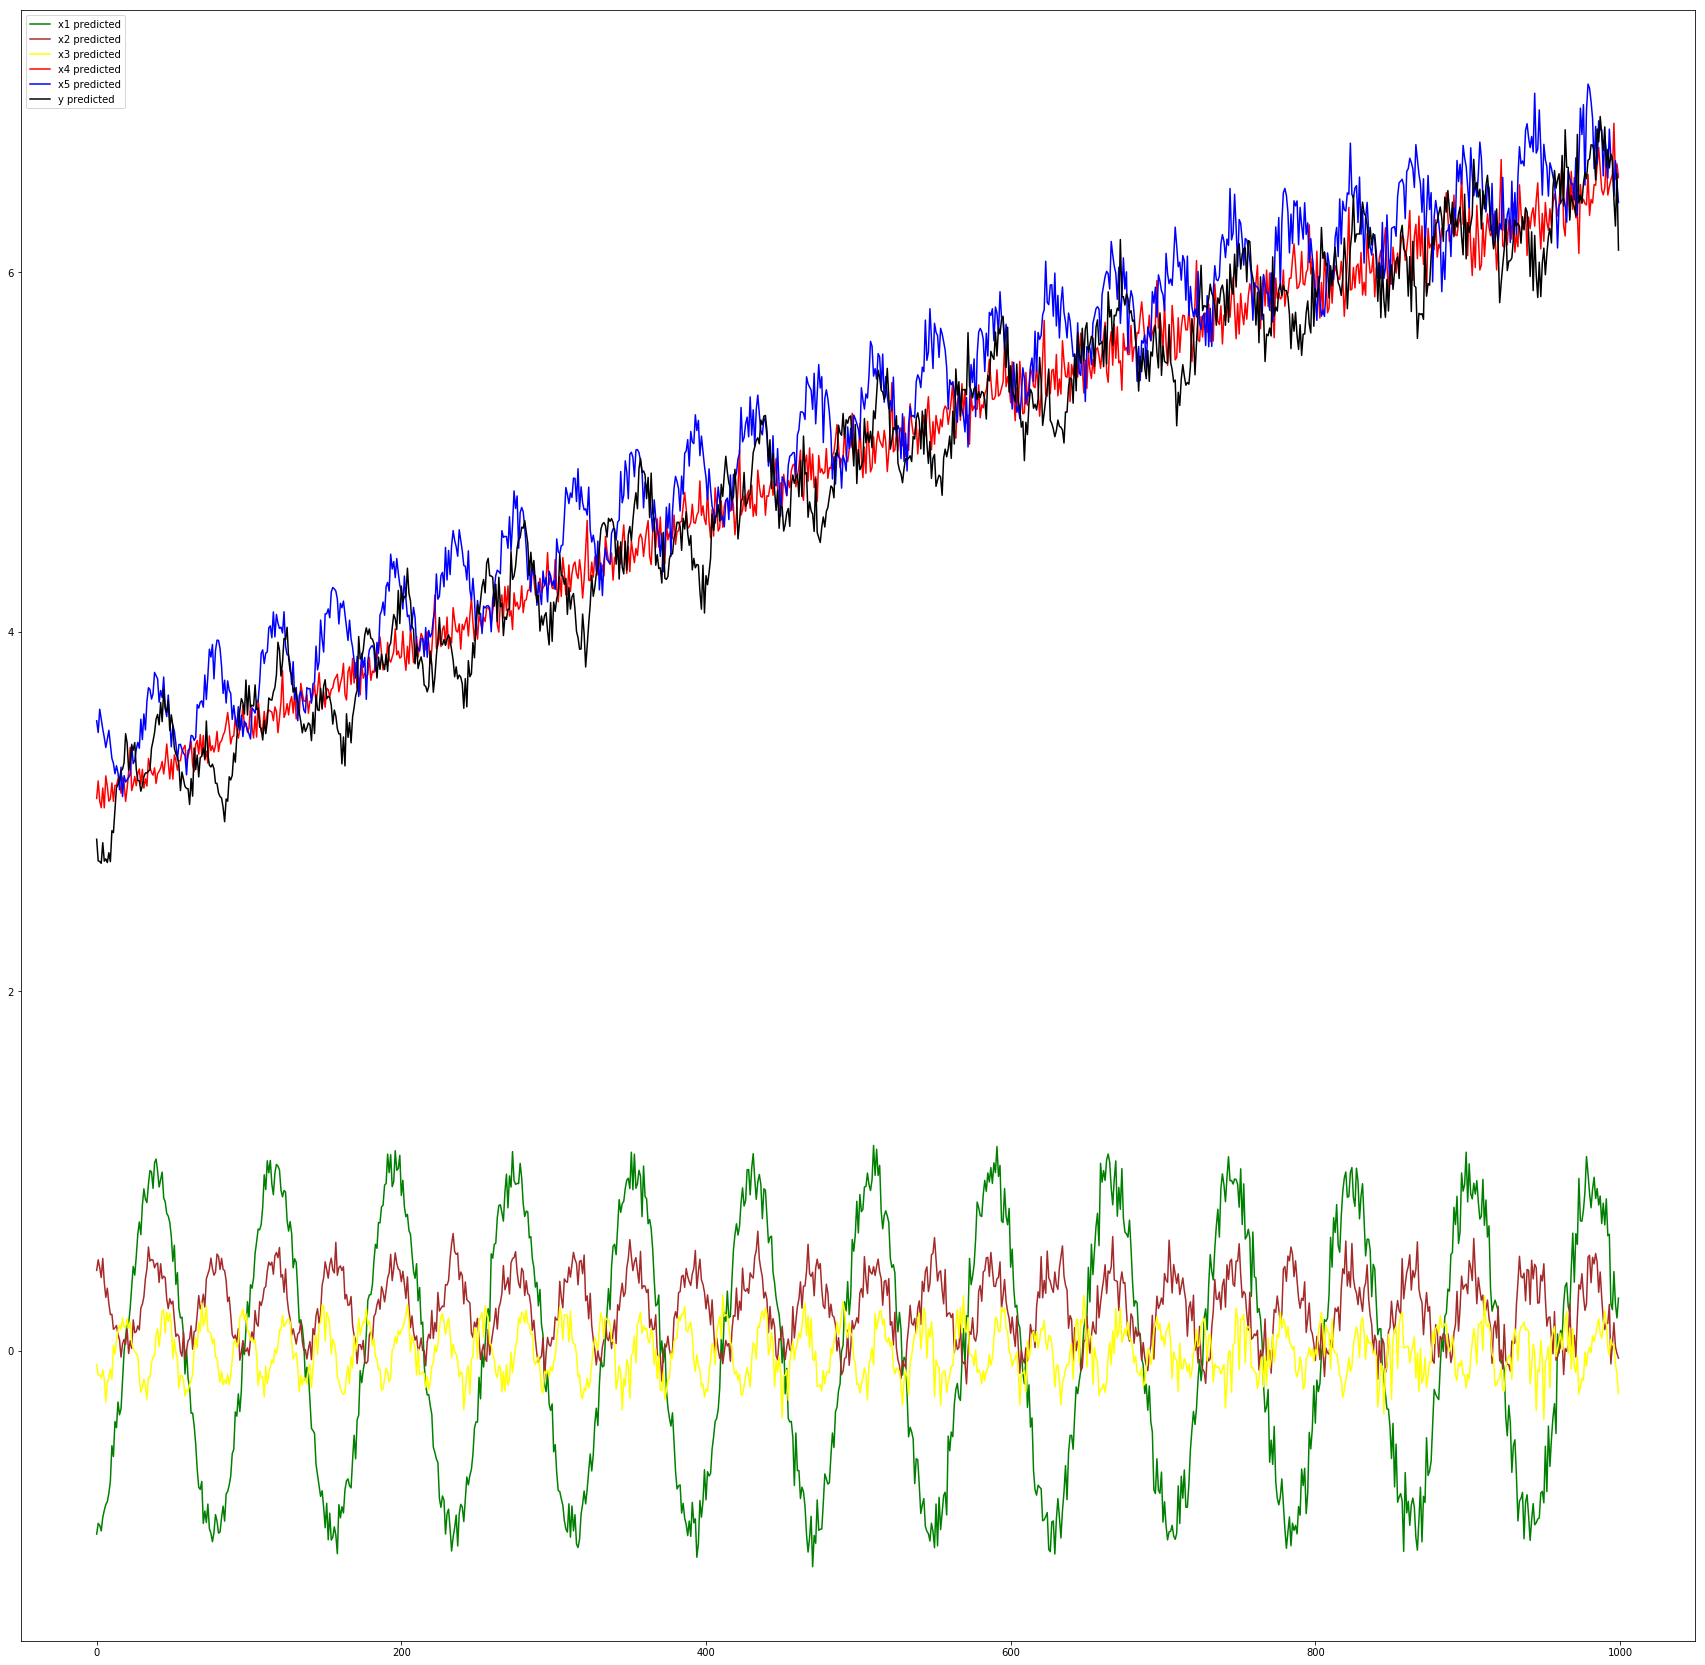
\includegraphics[width=0.9\textwidth]{./img/lstm_only_prediction.png}
% 	\caption{LSTM only model prediction}
% 	\label{img:lstm_only_prediction}
% \end{figure}

% \section{Влияние гиперпараметров модели на качество предсказаний}

% % todo
% % Посмотреть, как карта будет самобалансироваться, если сделать прикольную обратную связь.

% При уменьшении количества эпох обучения, карта может расходиться, даже карта с осмысленными связями.

% Увеличение параметра $ n\_steps\_in $, количество предыдущих значений временных рядов,
% а так же размерность скрытого состояния увеличивают количество требуемой для обучения
% памяти не более, чем линейно каждый. Конкретный показатель роста будет зависеть от
% плотности связей в карте.
% Уменьшение этих параметров, позволяет сэкономить память и ускорить обучение,
% но страдает качество предсказаний.


\section{Выводы}

В данной главе была реализована система для автоматического когнитивного картирования с использованием
методов нейронных сетей.
Также описаны инструменты, с помощью которых была реализована система.
Описана структура программного обеспечения, проведено тестирование разработанной системы.
На основе тестирования была дана оценка реализованной системе.

% Следует перечислить, какие практические результаты были получены, а именно: какое программное или иное обеспечение было создано. В число результатов могут входить, например, методики тестирования, тестовые примеры (для проверки корректности/оценки характеристик тех или иных алгоритмов) и др. По каждому результату следует сделать вывод, насколько он отличается от известных промышленных аналогов и исследовательских прототипов.

